\documentclass[11pt, a4paper]{article}		% general format


%%%% Charset
\usepackage[utf8]{inputenc}					% use utf8					
\usepackage[russian]{babel}					% use russian font


%%%% Math
\usepackage{amsmath}						% Amer­i­can Math­e­mat­i­cal So­ci­ety (AMS) math fa­cil­i­ties
\usepackage{amsfonts}						% fonts from the AMS
\usepackage{amssymb}						% additional math symbols


%%%% Graphics
\usepackage{graphicx}


\author{Дедков Сергей}
\title{Отчет по лабораторной работе №7 :\\ Сервис тестирования корректности настройки SSL на сервере Qualys SSL Labs – SSL Server Test}
\date{2015}

%---------------------------------------------------------

\begin{document}
\maketitle
\tableofcontents
\newpage

%---------------------------------------------------------


\section{Цель работы}


%---------------------------------------------------------

\section{Ход работы}


%---------------------------------------------------------

\subsection{Изучить лучшие практики по развертыванию SSL/TLS}

\begin{itemize}

\item Приватный ключ и сертификат

\item Используйте 2048-битные закрытые ключи

\item Защитите закрытый ключ

\item Обеспечьте охват всех используемых доменных имен

\item Приобретайте сертификаты у надежного удостоверяющего центра

\item Используйте надежные алгоритмы подписи сертификата

\item Используйте безопасные протоколы

\item Используйте безопасные алгоритмы шифрования

\item Контроль за выбором алгоритма шифрования

\item Поддержка Forward Secrecy.

\item Отключите Renegotiation по инициативе клиента

\item Отключите TLS compression

\item Отключите RC4

\item Будьте в курсе атаки BEAST

\item Отключить SSL v3

\end{itemize}


%---------------------------------------------------------

\subsection{Изучить основные уязвимости и атаки на SSL последнего времени – POODLE, HeartBleed}

\begin{itemize}

\item POODLE 

Специалист по безопасности Бодо Мёллер (Bodo Möller) с коллегами из компании Google опубликовал подробности об уязвимости в дизайне протокола SSL 3.0. Уязвимость под кодовым названием POODLE («пудель», Padding Oracle On Downgraded Legacy Encryption, CVE-2014-3566) позволяет расшифровать содержимое защищённого канала коммуникации. В общем, на всех системах нужно срочно блокировать использование SSL 3.0, потому что работающего способа обойти эксплоит не существует.

SSL 3.0 (RFC6101), использующий шифр RC4, устарел примерно на 15 лет. На замену ему создали TLS 1.0, TLS 1.1 и TLS 1.2, но он до сих пор широко используется в браузерах, веб-серверах и т.д. И многие реализации TLS обратно совместимы с SSL 3.0.

Злоумышленник может умышленно принудить клиента подключиться именно по SSL 3.0, эмулируя разрывы связи, и после этого эксплуатировать уязвимость.

Google пишет, что для защиты достаточно отключить поддержку SSL 3.0 или шифрования в режиме сцепления блоков (CBC mode). Однако, в этом случае возникнут серьёзные проблемы с совместимостью. Поэтому рекомендуемый способ обхода — поддержка механизма TLS\_FALLBACK\_SCSV, который не позволяет злоумышленнику снизить защиту канала до SSL 3.0. Механизм также предотвращает снижение защиты с TLS 1.2 до 1.1 или 1.0, что может помочь в предотвращении будущих атак.

Браузер Chrome и серверы Google поддерживают TLS\_FALLBACK\_SCSV с февраля, так что есть достаточно доказательств, что метод действительно эффективен.

Дополнительно, для Google Chrome также представили патч, который не позволяет соединяться по SSL 3.0. Аналогичная опция появится в Firefox 34, который ожидается к выходу 25 ноября: там поддержку SSL 3.0 отключат по умолчанию.

\item HeartBleed

Ошибка (переполнение буфера) в криптографическом программном обеспечении OpenSSL, позволяющая несанкционированно читать память на сервере или на клиенте, в том числе для извлечения закрытого ключа сервера. Информация об уязвимости была опубликована в апреле 2014 года, ошибка существовала с конца 2011 года.

Heartbeat-пакет состоит из данных, которые сервер должен вернуть в неизменном виде (это гарантирует, что сервер расшифровывал пакет), и случайных заполняющих байтов. OpenSSL не проверял корректность этого пакета: возможен, например, пакет длиной 16 байт, в котором написано, что длина данных 64 килобайта (поле размера двухбайтовое). Подверженные ошибке версии OpenSSL выходили за пределы буфера и передавали клиенту столько памяти, сколько он запросил, позволяя атакующему получать не предназначенные для этого данные. RFC предписывает не отвечать на такие «отравленные» пакеты.

\end{itemize}


%---------------------------------------------------------

\subsection{Обзор домена из списка Recent Best}

Выбранный домен: encoredentalplan.com (198.39.202.30)

\begin{figure}[h!]
\centering
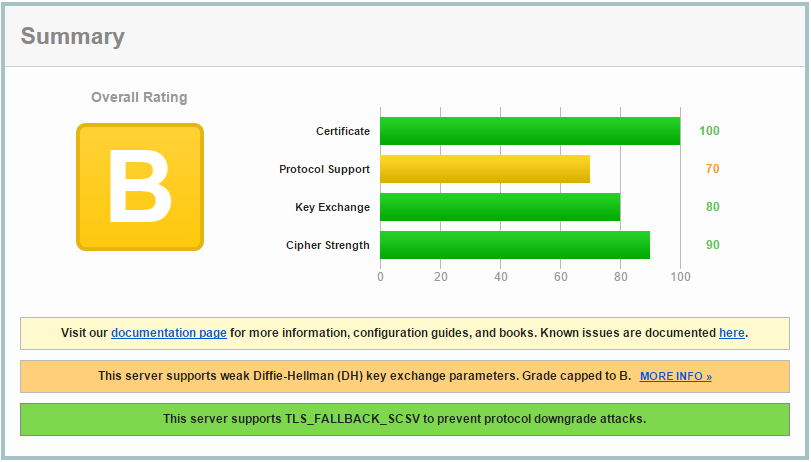
\includegraphics[scale=0.8]{res/summary_best_domain}
\caption{Summary домена из списка Recent Best}
\end{figure}

Общий рейтинг обозначается буквами A-F. В данном случае оценка домену выставлена B. В разделе summary можно увидеть выставенные оценки по 4 параметрам: Сертификат, Поддержка протокола, Обмен ключами, Стойкость шифра. (см. рисунок 1)

В пояснительной информации ниже указано почему оценка была снижена до B - слабые параметры протокола Диффи — Хеллмана. Значит может быть проведена атака Logjam Attack.

Так же указано, что сервер поддерживает TLS\_FALLBACK\_SCSV, который не позволяет злоумышленнику снизить защиту канала до SSL 3.0. Механизм также предотвращает снижение защиты с TLS 1.2 до 1.1 или 1.0, что может помочь в предотвращении будущих атак.

Из прочей информации можно отметить следующее(см. рисунок 2):

\begin{itemize}

\item Присутствуют слабые наборы шифров.

\item На некторых платформах обнаружены несоответствия

\end{itemize}

\begin{figure}[h!]
\centering
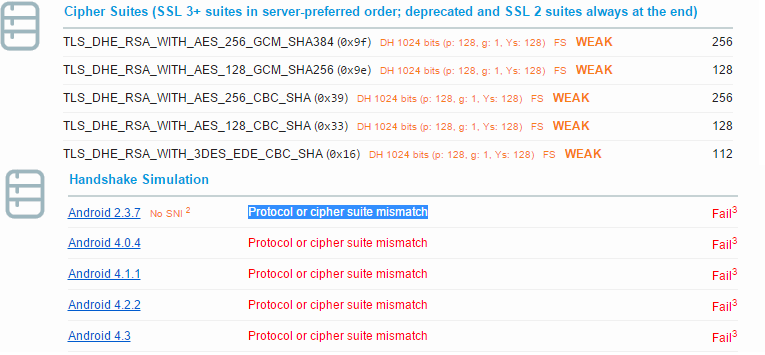
\includegraphics[scale=0.8]{res/info_best_domain}
\caption{Прочая информация домена из списка Recent Best}
\end{figure}



%---------------------------------------------------------

\subsection{Обзор домена из списка Recent Worst}

Выбранный домен: receiver.tvc.org (67.51.200.102)

\begin{figure}[h!]
\centering
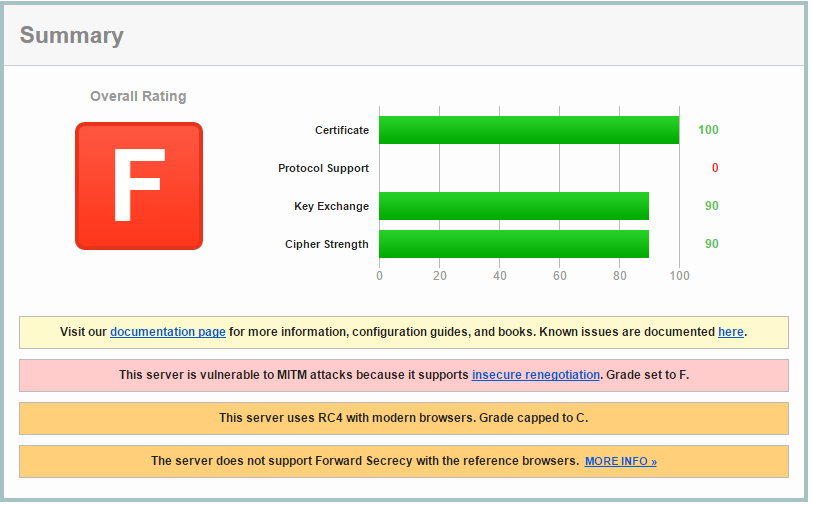
\includegraphics[scale=0.8]{res/summary_worst_domain}
\caption{Summary домена из списка Recent Worst}
\end{figure}

Аналогично предыдущему примеру можно увидеть оценки по 4м параметрам. (см. рисунок 3)

Из пояснительной информации:

\begin{itemize}

\item The server does not support Forward Secrecy with the reference browsers.

Домен не поддерживает прямую секретность, следовательно не гарантирует, что сессионные ключи, полученные при помощи набора ключей долговременного пользования, не будут скомпрометированы при компрометации одного из долговременных ключей.
С алгоритмами шифрования, которые не поддерживают Forward Secrecy, возможно расшифровать ранее зашифрованные разговоры с помощью закрытого ключа сервера. Нужно поддерживать и предпочитать ECDHE (аббревиатура ECDHE расшифровывается как «эфемерный алгоритм Диффи-Хеллмана с использованием эллиптических кривых») алгоритмы шифрования. Для поддержки более широкого круга клиентов, необходимо также использовать DHE, как запасной вариант после ECDHE.

\item This server uses RC4 with modern browsers. Grade capped to C.

Алгоритм RC4 является небезопасным и должен быть отключен. В настоящее время известно, что для взлома RC4 требуются миллионы запросов, много пропускной способности и времени. Таким образом, риск все еще относительно невелик, но вполне возможно, что атаки будут масштабнее в будущем. Если снимать RC4 нужно заранее проверить, будут ли существующие пользователи затронуты; другими словами, проверить, есть ли клиенты, которые поддерживают только RC4.

\item This server is vulnerable to MITM attacks because it supports insecure renegotiation. Grade set to F.

Сервер поддерживает небезопасное пересогласование ключей, отчего возможны ткие типы атак, как Cross-Site Request Forgery и Cross-Site Scripting.

\end{itemize}

Прочую информацию можно увидеть на рисунке 4.

\begin{figure}[h!]
\centering
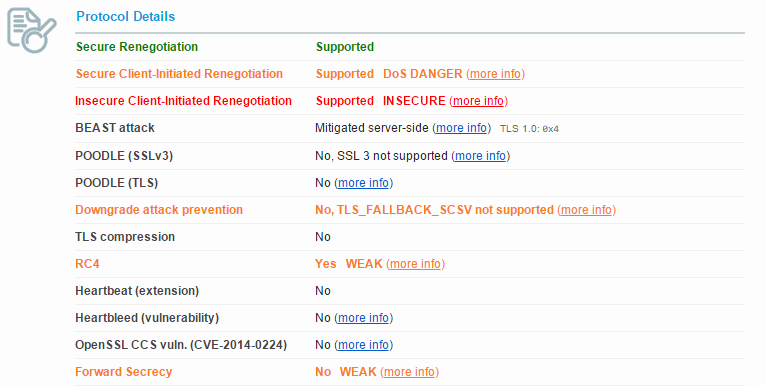
\includegraphics[scale=0.8]{res/info_worst_domain}
\caption{Прочая информация домена из списка Recent Worst}
\end{figure}

%---------------------------------------------------------

\subsection{Обзор известного сайта по выбору}

Выбранный домен: rzd.ru (217.175.140.90)

%---------------------------------------------------------

\subsubsection{Интерпретировать результаты в разделе Summary}

На рисунке 5 можно увидеть резуьтаты и оценки проверки.


\begin{figure}[h!]
\centering
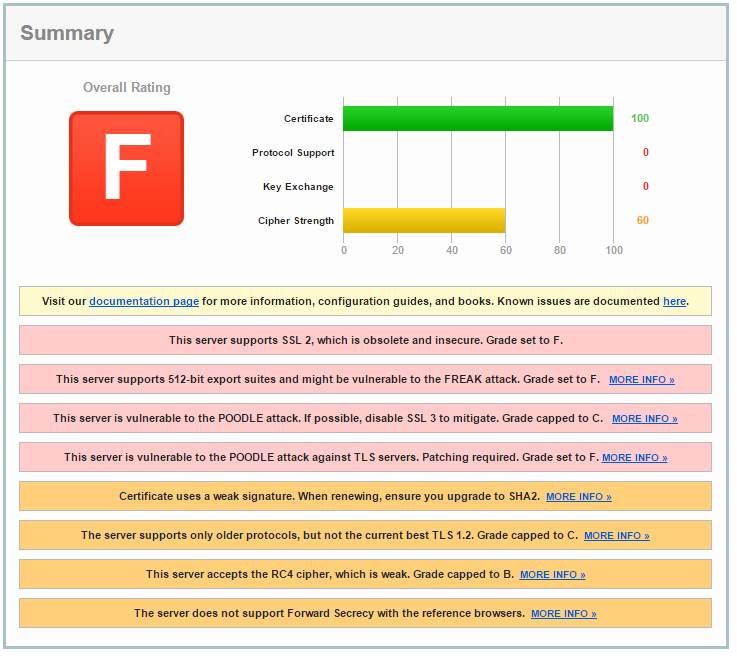
\includegraphics[scale=0.8]{res/summary_rzd}
\caption{Summary rzd.ru}
\end{figure}

Из пояснительной информации(описание раньше не встречавшихся замечаний):

\begin{itemize}

\item The server supports only older protocols, but not the current best TLS 1.2. Grade capped to C.

На рисунке 6 можно увидеть, что на сервере не поддерживается TLS 1.2 и TLS 1.1, зато поддерживается TLS 1.0, SSL 3, SSL 2.
При этом SSL 3 и SSL 2 считаются незащищенными.

\begin{figure}[h!]
\centering
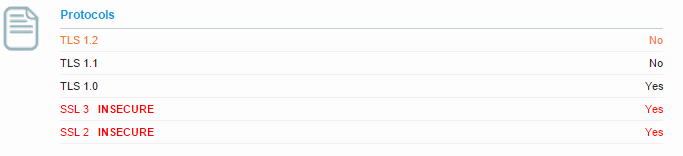
\includegraphics[scale=0.8]{res/protocols_rzd}
\caption{Protocols rzd.ru}
\end{figure}

\item Certificate uses a weak signature. When renewing, ensure you upgrade to SHA2.

Используемый алгоритм подписи на сервере: SHA1. Это можно увидеть в разделе Authentification. (см. рисунок 7)

\begin{figure}[h!]
\centering
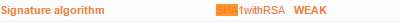
\includegraphics[scale=0.8]{res/signature_rzd}
\caption{Алгоритм подписи rzd.ru}
\end{figure}

Т.к. SHA1 считается небезопасным алгоритмом шифрования, предлагается обновить его на более современный и криптостойкий SHA2. 

\item This server is vulnerable to the POODLE attack. If possible, disable SSL 3 to mitigate. Grade capped to C. This server is vulnerable to the POODLE attack against TLS servers. Patching required. Grade set to F.

В виду того, что используется SSL шифрование на сервер можно осуществить атаку POODLE(см. выше). Так же возможно осуществлять атаку на сервер, где используется TLS(для некоторых реализаций), как в данном случае.

\item This server supports 512-bit export suites and might be vulnerable to the FREAK attack. Grade set to F.

Возможность FREAK атаки. азвание уязвимости «атака FREAK» происходит от фразы «Factoring attack on RSA-EXPORT Keys», означающей способ подбора открытых ключей к «экспортному» шифрованию RSA. Суть уязвимости заключается в том, что злоумышленнники могут заставить браузеры использовать более слабое шифрование, чем принято обычно. Тогда они смогут взломать его за считанные часы, получив не только доступ к чужим личным данным, но и возможность управлять содержимым страниц в браузере вплоть до кнопки лайка Фейсбука.

Причина появления FREAK лежит в старом требовании властей США, принятом ещё в 1990-е годы. После внедрения шифрования в браузер от Netscape государство требовало от технологических компаний оставлять в своих алгоритмах шифрования «лазейку» для спецслужб при экспортировании своих продуктов за рубеж.

Агентства вроде АНБ и ФБР опасались, что не смогут расшифровать слишком стойкий шифр, если понадобится вести слежку за пользователями в других странах. Несмотря на то, что требование не применять сильную криптозащиту в «экспортных» продуктах было снято в конце 1990-х, более слабое шифрование было интегрировано в множество программ и оставалось незамеченным публикой до недавнего времени.

«Экспортное» шифрование использовало ключи безопасности длиной в 512 бит, а не 1024, как было принято обычно. По данным исследователей, такой ключ можно было подобрать в течение семи часов при помощи мощности 75 обычных компьютеров или аренды аналогичной мощности за 100 долларов в «облачном» сервисе вроде Amazon Web Services. Демонстрацию подбора 512-битного ключа впервые публично провели в 1999 году.

\item This server supports SSL 2, which is obsolete and insecure. Grade set to F.

Поддержка SSL2, который считается устаревшим и не безопасным.

\end{itemize}

%---------------------------------------------------------

\subsubsection{Расшифровать все аббревиатуры шифров в разделе Configuration}

На рисунке 8 приведены испольхуемые шифры. Ниже расшифровка аббревиатур:

\begin{figure}[h!]
\centering
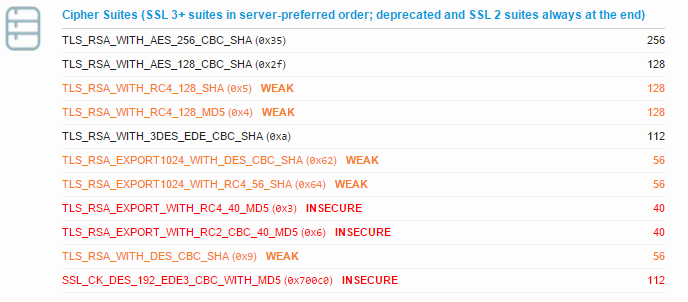
\includegraphics[scale=0.8]{res/cipher_suites_rzd}
\caption{Ипользуемые шифры rzd.ru}
\end{figure}

\begin{itemize}

\item TLS (англ. Transport Layer Security — безопасность транспортного уровня), как и его предшественник SSL (англ. Secure Sockets Layer — уровень защищённых сокетов) — криптографические протоколы, обеспечивающие защищённую передачу данных между узлами в сети Интернет[1]. TLS и SSL используют асимметричную криптографию для аутентификации, симметричное шифрование для конфиденциальности и коды аутентичности сообщений для сохранения целостности сообщений.

\item SSL (англ. secure sockets layer — уровень защищённых сокетов) — криптографический протокол, который подразумевает более безопасную связь. Он использует асимметричную криптографию для аутентификации ключей обмена, симметричное шифрование для сохранения конфиденциальности, коды аутентификации сообщений для целостности сообщений. 

\item RSA (аббревиатура от фамилий Rivest, Shamir и Adleman) — криптографический алгоритм с открытым ключом, основывающийся на вычислительной сложности задачи факторизации больших целых чисел. Криптосистема RSA стала первой системой, пригодной и для шифрования, и для цифровой подписи. Алгоритм используется в большом числе криптографических приложений, включая PGP, S/MIME, TLS/SSL, IPSEC/IKE и других.

\item Advanced Encryption Standard (AES), также известный как Rijndael — симметричный алгоритм блочного шифрования (размер блока 128 бит, ключ 128/192/256 бит), принятый в качестве стандарта шифрования правительством США по результатам конкурса AES. 

\item Режим сцепления блоков шифротекста (англ. Cipher Block Chaining, CBC) — один из режимов шифрования для симметричного блочного шифра с использованием механизма обратной связи. Каждый блок открытого текста (кроме первого) побитово складывается по модулю 2 (операция XOR) с предыдущим результатом шифрования.

\item Secure Hash Algorithm 1 — алгоритм криптографического хеширования. Описан в RFC 3174. Для входного сообщения произвольной длины (максимум $2^{64}-1$ бит, что примерно равно 2 эксабайта) алгоритм генерирует 160-битное хеш-значение, называемое также дайджестом сообщения. Используется во многих криптографических приложениях и протоколах. 

\item RC4 (англ. Rivest cipher 4 или англ. Ron’s code, также известен как ARCFOUR или ARC4 (англ. alleged RC4)) — потоковый шифр, широко применяющийся в различных системах защиты информации в компьютерных сетях (например, в протоколах SSL и TLS, алгоритмах обеспечения безопасности беспроводных сетей WEP и WPA).

\item MD5 (англ. Message Digest 5) — 128-битный алгоритм хеширования, разработанный профессором Рональдом Л. Ривестом из Массачусетского технологического института (Massachusetts Institute of Technology, MIT) в 1991 году. Предназначен для создания «отпечатков» или дайджестов сообщения произвольной длины и последующей проверки их подлинности.

\item Triple DES (3DES) — симметричный блочный шифр, созданный Уитфилдом Диффи, Мартином Хеллманом и Уолтом Тачманном в 1978 году на основе алгоритма DES, с целью устранения главного недостатка последнего — малой длины ключа (56 бит), который может быть взломан методом полного перебора ключа. 

\end{itemize}


%---------------------------------------------------------

\subsubsection{Прокомментировать большинство позиций в разделе Protocol Details}

Прокомментируем позиции в разделе Protocol Details. (см. рисунок 9)

\begin{figure}[h!]
\centering
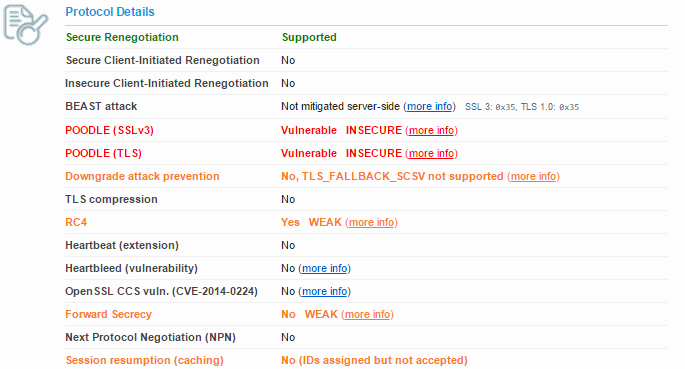
\includegraphics[scale=0.8]{res/protocol_details_rzd}
\caption{Описани протокола rzd.ru}
\end{figure}

\begin{itemize}

\item Secure Renegotiation - Supported.

Сервер поддерживает безопасное пересогласование ключей.

\item POODLE (SSLv3)	Vulnerable   INSECURE (more info), POODLE (TLS)	Vulnerable   INSECURE (more info),Downgrade attack prevention	No, TLS\_FALLBACK\_SCSV not supported (more info)

Существует поддержка SSL3, и при этом не установлен механизм TLS\_FALLBACK\_SCSV. Таким образом клиент может соединиться с сервером используя SSL3, в этом случае может быть использована атака POODLE.

\end{itemize}

Прочие моменты комментировались выше.

%---------------------------------------------------------

\subsubsection{Сделать итоговый вывод о реализации SSL на заданном домене}

Как видно из оценки и прочих данных реализация SSL на сайте rzd.ru не очень хороша. Существует ряд уязвимостей и атак, которыми могут воспользоваться злоумышленники.

%---------------------------------------------------------

\section{Вывод}

В результате выполнения работы были изучены лучшие практики по развертыванию SSL, возможные уязвимости. Получен опыт использования инструмента тестирования SSL на сервере (SSL Server Test). Помимо этого в ходе обнаружения недостатков серверов были изучены какие типы атак могут быть соверены на них, причины этого и каким образом можно предотвращать эти атаки.

\end{document}